\documentclass{article}
\usepackage{amsmath,amsfonts,amsthm,graphicx,geometry,url,wrapfig}
\usepackage{array}
\usepackage{sectsty}							
\usepackage[svgnames]{xcolor}
\usepackage{multirow} 
\usepackage{dashrule}
\usepackage{arydshln}

\sectionfont{									
		\usefont{OT1}{phv}{b}{n}%					
		\sectionrule{0pt}{0pt}{-3pt}{3pt}
		}

\newcommand{\sepspace}{\vspace*{1em}}		

\newcommand{\MyName}[1]{
		\huge \usefont{OT1}{phv}{b}{n} \hfill #1 		
		\par \normalsize \normalfont
		}

\newcommand{\NewPart}[1]{\section*{\uppercase{#1}}}

\newcommand{\SkillsEntry}[2]{						
		\noindent\hangindent=2em\hangafter=0 		
		\parbox{\spacebox}{						
		\textit{#1}}								
		\hspace{1.5em} #2 \par
		}					
		
\newcommand{\EducationEntry}[4]{
		\noindent \textbf{#1} \hfill 	{#2} \par				
		\noindent \textit{#3} \par	
		\noindent #4 	
		\normalsize \par
		}
		
\newcommand{\ScholasticAcheivements}[4]{
		\noindent \textbf{#1} \hfill \textbf{#2} \\
		\textit{#3}	 \hfill	 \textit{ #4} 	
		\normalsize \par
		}
		
\newcommand{\WorkEntry}[4]{						
		\noindent \textbf{#1} \hfill 					
		\colorbox{Black}{\color{White}#2} \par		
		\noindent \textit{#3} \par					
		\noindent\hangindent=2em\hangafter=0 \small #4 	
		\normalsize \par
		}

\newcommand{\transcriptentry}[6]{
		\tiny{#1} & \tiny{#2} & \tiny{#3} & \tiny{#4} & \tiny{#5} & \tiny{#6} \\ 
		}		

%------------------------------------------mera photo................................................................%
\begin{document}
\begin{wrapfigure}{l}{0.5\textwidth}
	\vspace*{-2em}
		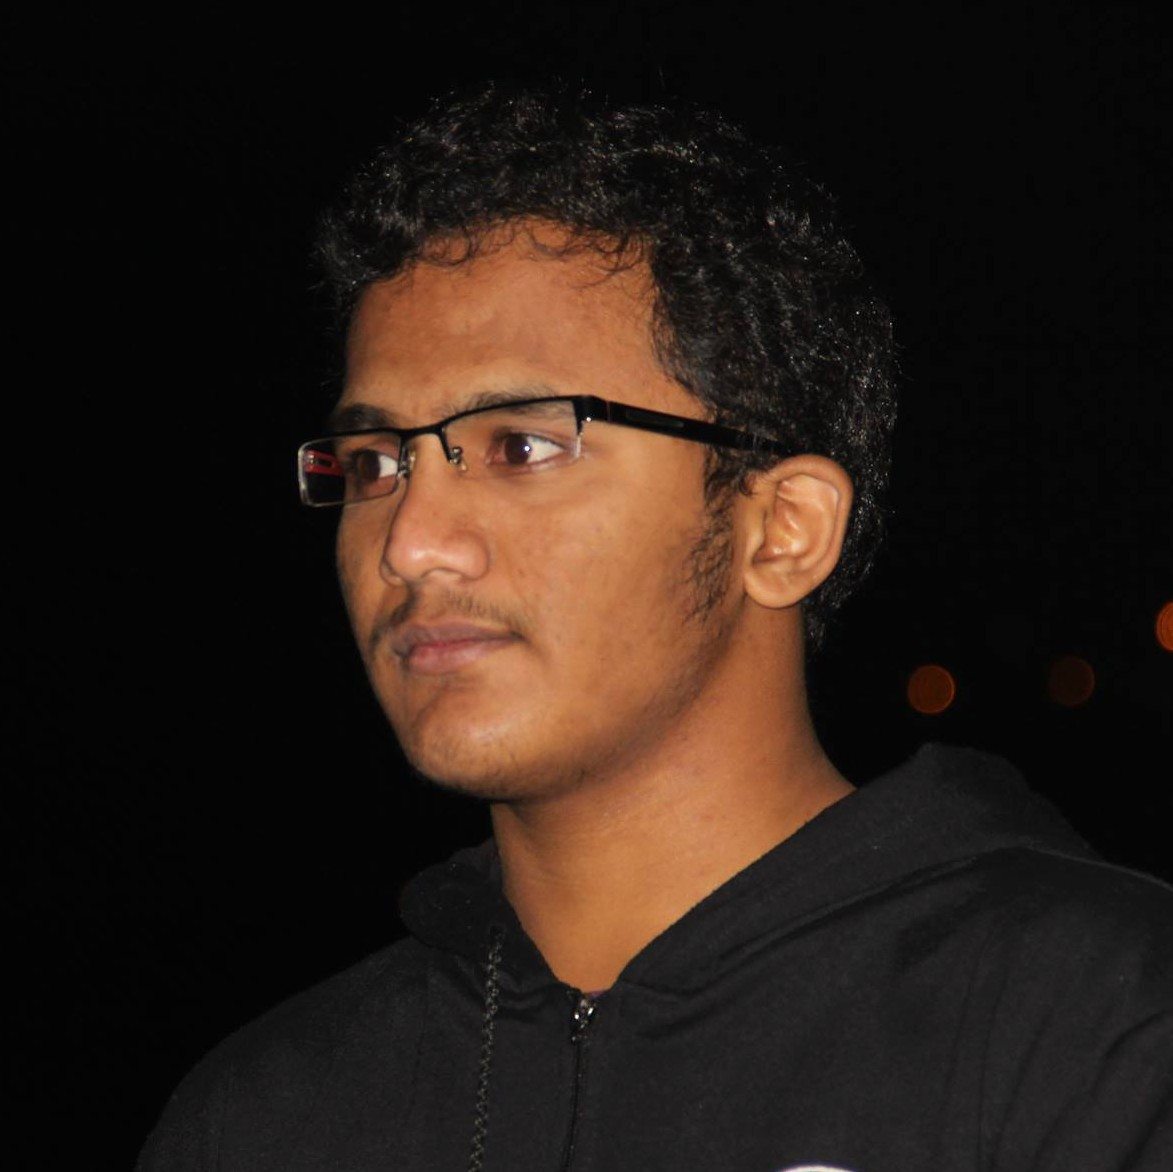
\includegraphics[width=0.25\textwidth]{photo.jpg}
\end{wrapfigure}
%................................................end..................................................................%

%..............................................Personal Details.........................................................%
\MyName{Manikanta Reddy D}
\begin{flushright}
	$2^{nd}$ year undergraduate\\
	Dept. of Computer Sciences\\
	Indian Institue of Technology, Kanpur
\end{flushright}
%..............................................end......................................................................%

\sepspace

%..........................................EDU INFO....................................................................%
\NewPart{Education}{}

\EducationEntry{B.Tech, Computer Sciences}{2013-}{Indian Institute of Technology, Kanpur}{\emph{performance : 8.0/10.0}}

\sepspace

\EducationEntry{Intermediate}{2011-2013}{Sri Chaitanya Narayana Group, Hyderabad}{\b{\emph{performance : 96.9/100}}}

\sepspace

\EducationEntry{High School}{2000-2011}{Sri Chaitanya Group, Hyderabad}{\b{\emph{performance : 94.3/100}}}

\sepspace
%............................................end............................................................%

%......................................ACH ZONE.............................................................%
\NewPart{Scholastic Acheivements}{}

\ScholasticAcheivements{AIR 121}{Gold Medal}{IIT-JEE, 2013}{IGNOU-SAARC Olympiad, 2011}

\sepspace

\ScholasticAcheivements{KVPY Scholar}{Aditya Birla Scholarship}{Placed 37th in CML, 2011}{Nominated in 2013}

\sepspace
%.............................................end.......................................................%

%.......................................TRANSCRIPT ZONE.................................................%
\begin{center}
	\tiny{INDIAN INSTITUTE OF TECHNOLOGY}\\
	\tiny{GRADE REPORT}\\
	\tiny{ROLL NO : 13265} \hfill \tiny{DEPARTMENT : COMPUTER SC. \& ENGG.}\\
	\tiny{NAME : DORNALA MANIKANTA REDDY} \hfill \tiny{PROGRAM : BACHELOR OF TECHNOLOGY}\\
\end{center}
\begin{center}
	\begin{tabular}{m{5em}  m{1.5cm} m{5cm} m{0.5cm} m{0.7cm} m{0.3cm} m{0.5cm}} 
	\hdashline
	\tiny{\textbf{YEAR/SEM}} & \transcriptentry{\textbf{COURSE}}{\textbf{TITLE}}{\textbf{UNIT}}{\textbf{GRADE}}{\textbf{SPI}}{\textbf{CPI}}
	\hdashline
	\multirow{7}{5em}{\tiny{2013-2014 FIRST}}
		& \transcriptentry{CHM101A}{CHEMISTRY\,LABORATORY}{3}{A}{}{}
		& \transcriptentry{ESC101A}{FUNDAMENTALS\,OF\,COMPUTING}{14}{B}{}{}
		& \transcriptentry{MTH101A}{MATHEMATICS\,I}{11}{B}{}{}
		& \transcriptentry{PE101A}{MORNING\,EXERCISE}{3}{S}{}{}
		& \transcriptentry{PHY103A}{PHYSICS\,II}{11}{C}{}{}
		& \transcriptentry{PSY151A}{INTRODUCTION\,TO\,PSYCHOLOGY}{11}{B}{}{}
		& \transcriptentry{}{}{}{}{7.7}{7.7}
		\\
	\multirow{7}{5em}{\tiny{2013-2014 SECOND}}
		& \transcriptentry{CHM102A}{GENERAL\,CHEMISTRY}{8}{B}{}{}
		& \transcriptentry{LIF101A}{INTRODUCTION\,TO\,BIOLOGY}{6}{B}{}{}
		& \transcriptentry{MTH102A}{MATHEMATICS\,II}{11}{B}{}{}
		& \transcriptentry{PE102A}{EVENING\,EXERCISE}{3}{S}{}{}
		& \transcriptentry{PHY101A}{PHYSICS\,LABORATORY}{3}{B}{}{}
		& \transcriptentry{PHY102A}{PHYSICS\,I}{11}{A}{}{}
		& \transcriptentry{TA101A}{ENGINEERING\,GRAPHICS}{9}{A}{}{}
		& \transcriptentry{}{}{}{}{8.8}{8.2}
		\\	
	\multirow{7}{5em}{\tiny{2014-2015 FIRST}}
		& \transcriptentry{COM200}{COMMUNICATIONS\,SKILLS:\,COMPOSITION}{5}{S}{}{}
		& \transcriptentry{CS201A}{MATHEMATICS\,FOR\,COMPUTER\,SCIENCE-I}{9}{C}{}{}
		& \transcriptentry{CS210A}{DATA\,STRUCTURES\,AND\,ALGORITHMS}{12}{B}{}{}
		& \transcriptentry{ESC201A}{INTRODUCTION\,TO\,ELECTRONICS}{14}{B}{}{}
		& \transcriptentry{ES0202A}{MECHANICS\,OF\,SOLIDS}{11}{B}{}{}
		& \transcriptentry{TA201A}{MANUFACTURING\,PROCESSES\,I}{6}{B}{}{}
		& \transcriptentry{}{}{}{}{7.7}{8.0}\\
	\hdashline
	\end{tabular}
\end{center}
%........................................end................................................................%

\end{document}